\section{Pourquoi passer à des solutions pair à pair?}
	\label{whyp2p}
	Nous allons savoir pourquoi est-il nécessaire de passer d'une architecture Client/Serveur à une architecture pair à pair, pour cela nous verrons les différences des deux solutions et les avantages d'une approche pair à pair.
	\subsection{Les solutions existantes}
	Dans la plupart des jeux en ligne massivement multi joueur, l'architecture est de type client/serveur (voir page ~\pageref{P2P/ClServ}). Dans cette architecture, il a une forte distinction entre le client, qui envoie des requêtes au serveur et attend les réponses, et le serveur qui est à l'écoute de requêtes des clients. Cette approche simplifie la sécurité et le fonctionnent global des jeux. Par exemple, pour effectuer des mises à jour sur l'état global du jeu, il suffit de le faire sur un seule machine ( le serveur principal) et il n'y a pas de problème d'incohérence entre les données. De même pour la sécurité, toutes les données étant regroupées sur une seule machine, le contrôle sera beaucoup plus simple que dans des systèmes distribués où le nombre de point d'entrée sera beaucoup plus important. \\
	Le problème de cette architecture est qu'elle ne passent pas à l'échelle sans mettre de gros moyen en terme de machines et donc financier, le serveur devient un goulot d'étranglement et si un trop grand nombre de joueurs se connecte, le serveur ne tiendra pas ~\cite{1198269}. Le problème est résolu "temporairement?" en ayant des serveurs de très grandes capacités ou en mettant en place des clusters de serveur \textbf{(voir bibli)}. Mais ces solutions induisent un gros investissement dès le début de la mise en service du jeu et le coût de maintenance est très élevé. Un autre problème est le disponibilité du système en cas de panne du serveur, si le serveur tombe en panne alors plus personne n'aura accès à l'application que ce dernier faisait fonctionner. \\
	Au vue du nombre croissant de participant à ce genre de jeux vidéos massivement multi joueur, le passage à l'échelle devient un sujet très important et c'est pour cela que les recherches sur des architectures distribuées sont de plus en plus importantes textbf{(voir si statistiques)}. \\
	\subsection{Les avantages et les inconvénients du pair à pair}
	Comme il est dit précédemment, l'augmentation croissante des recherches sur le sujet atteste du fait que des problématiques ressortent des solutions existantes. Le problème du passage à l'échelle est sûrement le plus important et est l'une des raisons principales de toutes ces recherches. Les architectures pair à pair ne font plus ressortir d'entité serveur et client comme nous le connaissions dans l'architecture client/serveur, chaque nœud sera client et serveur en fonction du temps et en fonction de ses besoins (voir page ~\pageref{P2P/ClServ}). Les systèmes pair à pair peuvent avoir une multitude d'utilisation, que ce soit dans le partage de fichier, la communication, les jeux vidéos , le calcul scientifique, le militaire, etc. \\
	L'architecture pair à pair est faite telle qu'il n'y a pas de goulot d'étranglement,car nous passons d'un système où tout passait par un point unique à un système qui comporte un grand nombre d'entité qui peuvent toutes avoir le même rôle. L'utilisation de l'architecture pair à pair peut entrainer un grand nombre de communications, elle nécessite des synchronisations des entités, de la gestion des ressources partagées et d'autres problèmes liés à la répartition des données, il faut donc trouver des solutions à tous ces problèmes éventuels. Le pair à pair est donc plus adapté à des applications massivement multi joueur mais il faudra pouvoir garantir les mêmes propriétés que les systèmes client/serveur. \\
	Les systèmes pair à pair sont par exemple plus difficile à surveiller, les phénomènes de tricherie sont donc plus difficile à surveiller, de même pour la sécurité. Nous avons pu voir qu'il existe trois type de tricherie: par Confidentialité, c'est à dire d'obtenir des informations non autorisées sur d'autres utilisateurs; par Intégrité, si il y des modifications du monde, des lois physiques ou les lois du jeu non autorisées; par Availability, c'est le fait de provoquer des ralentissements ou des arrêts de partie du jeu ( référence vers Challenges in P2P gaming). Il faut que le système soit aussi fiable sur le long terme et qu'il soit tolérant aux connexions et déconnexions.\\
	Les jeux vidéos sont des applications distribuées qui ne sont pas dites "critique", le fait que le jeu ralentisse un petit peu de manière très ponctuelle n'est pas gênant, certaines propriétés des applications distribuées peuvent être retardées ou sautées ponctuellement. Ils ont des avantages qui font qu'il sera plus aisé de réaliser une distribution~\cite{1267692}:
	\begin{itemize}
		\renewcommand{\labelitemi}{$\bullet$}
		\item Les jeux vidéos tolèrent une consistence faible pour les différents états de l'application.
		\item Il est assez aisé de prédire les écritures et les lectures grâce à l'ensemble des règles définies dans le jeu. 
	\end{itemize}
	\vspace{1cm}
	\begin{figure}[!h]
	\centering
	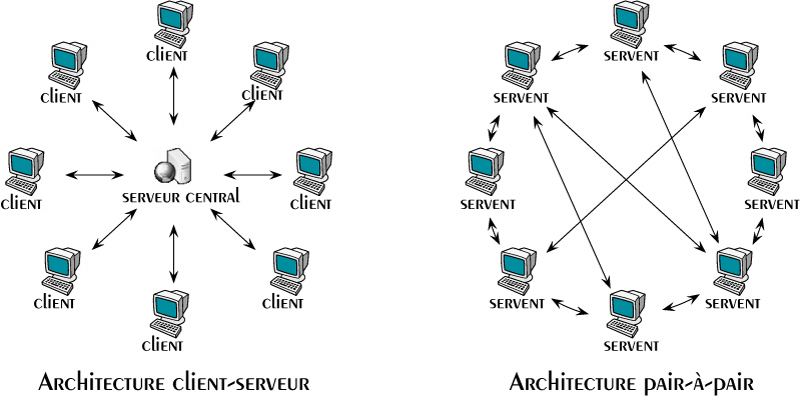
\includegraphics[width=12cm,height=6cm]{../Images/p2p-85145.png}\\
	\caption{Schéma des architectures pair à pair et client/serveur}
	\label{P2P/ClServ}
	\end{figure} 
\newpage
